\section{Lecture 4: The motion of projectiles}

Let's revisit this trajectory shown in \ref{fig:motion-of-projectiles}

For now, ignore the green parts, which are the location of the position vector after a certain time has passed.
Relevant equations for this trajectory can be written as

\begin{align}
x(t) &= (v_0 \cos \alpha) t \label{eq:lec3_x}\\
v_x(t) &= v_0 \cos \alpha\\
y(t) &= (v_0 \sin \alpha) t - \frac{1}{2} g t^2 \label{eq:lec3_y}\\
v_y(t) &= v_0 \sin \alpha - g t
\end{align}

where $v_0$ is the initial velocity diagonally, at angle $\alpha$ to the ground, and $g = +\SI{9.8}{m/s^2}$. Since $g$ is a positive number, we need to use a minus sign here: we have defined increasing $y$ to be upwards, but gravity accelerates downwards.\\
The first and third equations could have $x_0$ and $y_0$ terms, respectively, but we can choose the origin of our coordinate system to be the exact point from where the ball is thrown, which means we choose them both to equal zero.

We can write equation \eqref{eq:lec3_y} above in terms of $x$, instead of $t$, by solving \eqref{eq:lec3_x} for $t$ and making the substitution:

\begin{align}
x(t) &= (v_0 \cos \alpha) t\\
t &= \frac{x(t)}{v_0 \cos \alpha}
\end{align}

\begin{align}
y(t) &= (v_0 \sin \alpha) t - \frac{1}{2} g t^2\\
y(t) &= (v_0 \sin \alpha) \left(\frac{x(t)}{v_0 \cos \alpha}\right) - \frac{1}{2} g \left(\frac{x(t)}{v_0 \cos \alpha}\right)^2\\
     &= x(t) \tan \alpha - \frac{1}{2} g \frac{x(t)^2}{v_0^2 \cos^2 \alpha}
\end{align}

We can then see than this has the form of $x$ times a constant, minus $x^2$ times another constant.

\begin{equation}
y(t) = C_1 x - C_2 x^2
\end{equation}

In other words, the trajectory has the shape of a parabola.

We can calculate when the object reaches the maximum height (the apex of the trajectory), by setting the $v_y(t)$ equation equal to zero. The object is launched with an initial velocity, and will only ever stand ``still'' (on the $y$ axis) when it changes from going upwards to going downwards, since the equation doesn't capture what happens when it hits the ground, etc.

\begin{align}
v_0 \sin \alpha - g t_p = 0\\
g t_p = v_0 \sin \alpha\\
t_p = \frac{v_0 \sin \alpha}{g}
\end{align}

In other words, the time to reach the peak height is simply the initial velocity in the $y$ direction, divided by the acceleration that opposes that motion.\\
We can then find the highest point $h$ that it ever reaches, by substituting the time found above into the $y(t)$ equation:

\begin{align}
h &= (v_0 \sin \alpha) \frac{v_0 \sin \alpha}{g} - \frac{1}{2} g \left(\frac{v_0 \sin \alpha}{g}\right)^2\\
h &= \frac{v_0^2 \sin^2 \alpha}{g} - \frac{v_0^2 \sin^2 \alpha}{2g}\\
h &= \frac{v_0^2 \sin^2 \alpha}{g} \left(1 - \frac{1}{2}\right)\\
h &= \frac{(v_0 \sin \alpha)^2}{2g}\label{eq:lec3_height}
\end{align}

When $y=0$, $t$ will be the time the object lands on ground. We will also get $t=0$ since the trajectory
started at the origin O. A trick we can use since the trajectory starts at O and there is no air dag,
i.e., the parabola is semetrical. We can calculate the time to reach the highest position and multiply it by two.

\begin{align}
t_s = 2 t_p\\
t_s = \frac{2 v_0 \sin \alpha}{g}
\end{align}

Finally, we can calculate the distance OS, which is the horizontal distance traveled. (Not the entire distance of the parabola, i.e. the arc length!)\\
This distance is simply $v_{0x}$ times $t_s$, but that expression is slightly hairy. Let's write it down and then simplify it:

\begin{align}
\text{OS} = (v_0 \cos \alpha) \left(\frac{2 v_0 \sin \alpha}{g} \right)\\
\text{OS} = \frac{2 v_0^2 \sin \alpha \cos \alpha}{g}
\end{align}

$2 \sin \alpha \cos \alpha = \sin 2 \alpha$ via a trigonometric identity, so:

\begin{align}
\text{OS} = \frac{v_0^2 \sin 2\alpha}{g} \label{eq:lec3_os}
\end{align}

Thus, to maximize horizontal distance $\sin{2\alpha}$ should maximize, which it is when $2\alpha=90^{\circ}$.
Therefore, the horizontal distance is largest when $\alpha=45^{\circ}$


\subsection{Trajectory demonstrations}

By firing a small projectile we can demonstrate the trajectory. 
To calculate the horizontal distance we can use equation~\ref{eq:lec3_os},
but we need $v_0^2$ first which we can get from equation~\ref{eq:lec3_height}
which is derived to:
\begin{eqnarray*}
  v_0^2 &= \frac{2gh}{\sin^2 \alpha}
\end{eqnarray*}

However, we have to measure the height, which can be done firing straight up, i.e., $\alpha = \ang{90}$.
Giving us $v_0^2=2gh$. The professor measures max height to be approximately $h_{max}=3.07(15)$ with an error of $5\%$.
Thus, $v_0^2 = 2\cdot9.81\cdot\SI{3.07(15)}{m^2/s^2} =  \SI{60.2(30)}{m^2/s^2}$.

When we use an angle of $\ang{45}$ we get:
\begin{equation}
\ang{45}\text{ OS} = \frac{\SI{60.2}{m^2/s^2} \sin \ang{90}}{\SI{9.81}{m/s^2}} = \SI{6.14(31)}{m}
\end{equation}


\subsection{A story about a monkey}

No monkeys were hurt in the making of this demonstration!

Imagine a monkey, sitting in a tree. A short bit away, a hunter places a golf ball cannon, aimed directly at the monkey (dotted line, below).

\begin{figure}[H]
  \centering
\begin{tikzpicture}[scale=1.5]
  % Trajectory
  \draw[thick, domain=0:6.2, samples=100] 
      plot (\x, {0.8*\x - 0.1*\x^2}); % Parabolic trajectory
  
  % Mokey
  \node at (6, 4) {\Strichmaxerl[3]};
  \node at (6.4, 4.4) {$t_2$};

  % Brakets
  \draw [red, decorate, decoration = {brace}] (4.1, 2.7) -- (4.1, 1.6) node[midway, right] {$\frac{1}{2}gt_1^2$};
  \draw [red, decorate, decoration = {brace}] (6.2,4) -- (6.2, 1.2) node[midway, right] {$\frac{1}{2}gt_2^2$};

  \draw [dotted, green] (0,0) -- (6,4);
  \draw [dotted] (6,0) -- (6,4);
  \draw [dotted] (4,0) -- (4,2.7);
  \draw [thick] (0,0) -- (6,0);
  \node[green] at (2.3, 2.2) {no $g$};
  \node at (2.7, 1) {with $g$};
  \node at (7.1, 3.6) {$y_t$};

  \fill[black] (6, 1.2) circle (2pt) node[right=3mm] {$t_2$};
  \fill[black] (4, 1.6) circle (2pt) node[below left=1mm and 1mm] {$t_1$};
  \fill[black] (4, 2.7) circle (2pt) node[left=1mm] {$t_1$};

  % Vectors
  \draw [thick, red, -{Stealth[scale=1.5]}] (0, 0) -- (2, 1.4) node[above] {$v_0$};
  \draw [thick, red, -{Stealth[scale=1.5]}] (0, 0) -- (2, 0);
  \draw [thick, red, -{Stealth[scale=1.5]}] (0, 0) -- (0, 1.4);

  \draw[->, red] (0.9, 0) arc[start angle=0, end angle=45, radius=0.7];
  \node[text=red] at (1.1, 0.3) {$\alpha$};
  \draw [dotted, red] (2, 0) -- (2, 1.4);
  \draw [dotted, red] (0, 1.4) -- (2, 1.4);

\end{tikzpicture}
\end{figure}

Because the horizontal velocity is the same regardless of whether there is gravity, we know that at a certain time $t$, the golf ball will be at the same $x$ position regardless; only the height will differ.

The dotted line above shows how the ball would travel in the absence of gravity, while the filled line shows the parabolic trajectory it would take on Earth. As we can see, it falls a distance of $\frac{1}{2} g t_1^2$ during a time interval $t_1$ after being fired -- basic 1D kinematics.

Now, there's an additional crux in this problem: as soon as the monkey sees the cannon fire, he lets go and starts falling. The monkey will fall with exactly the same acceleration as the golf ball, and since they started falling at the same time, the golf ball will hit the poor monkey despite his attempt to flee. Had he instead stayed where he was, all would probably be well!

Note that this fact is independent of the golf ball's velocity, as long as it doesn't hit the ground before reaching the monkey's $x$ coordinate. High velocity or low velocity, the gravitational acceleration is the same regardless, and so the ball and the monkey will both fall the same vertical distance in a given amount of time.

Now, let's imagine that all of this happens inside an elevator, which is in free fall. Both the gun and the monkey (and the tree) accelerate downwards at $-g$.

\begin{figure}[H]
  \centering
\begin{tikzpicture}
  \draw[thick] (0,0) -- (5, 0) node[midway, below] {$D$};
  \draw[dotted] (0,0) -- (5, 3) node[midway, above, rotate = 30] {$\sqrt{D^2+h^2}$};
  \draw[red, -{Stealth[scale=1.5]}] (0,0) -- (1.6, 1.0) node[midway, above] {$v_0$};
  \draw [decorate, decoration = {brace}] (5, 3) -- (5, 0) node[midway, right] {$h$};

  \node[cylinder, 
	draw = black, 
	cylinder uses custom fill, 
	aspect = 0.2, 
  minimum height = 8mm,
	rotate = 30] {};

  \fill[black] (5,3) circle (3pt);
\end{tikzpicture}
\end{figure}

From the monkey's point of view, because he falls at the same acceleration and velocity as the gun, the golf ball comes straight at him, without any arcing. As shown above, as far as the monkey can see, the distance the ball has to travel is $\sqrt{D^2 + h^2}$, the hypotenuse of the triangle created by the horizontal distance to the cannon and the (vertical) height of the tree.

Considering the golf ball's velocity, from this point of view, the monkey will get hit in

\begin{equation}
t_{kill} = \frac{\sqrt{D^2 + h^2}}{v_0}
\end{equation}

seconds. However, from a different perspective (see the previous image above), we would instead calculate it as

\begin{equation}
t_{kill} = \frac{D}{v_0 \cos \alpha}
\end{equation}

since $v_0 \cos \alpha$ is the ball's velocity in the horizontal direction.\\
How come the two are not the same? Surely they must both agree? And they do. We can use the definition of $\cos \alpha$ in the above diagram:

\begin{equation}
\cos \alpha = \frac{D}{\sqrt{D^2 + h^2}}
\end{equation}

... and substitute that into what we had just above:

\begin{equation}
t_{kill} = \frac{D}{v_0 \frac{D}{\sqrt{D^2 + h^2}}} = \frac{\sqrt{D^2 + h^2}}{v_0} 
\end{equation}

and so the two agree on the timing of the monkey's unfortunate demise.

\newpage

\section{Lecture 5: Uniform circular motion}

Consider an object moving at a constant speed $v$ around a circle of radius $r$:

\begin{figure}[H]
  \centering
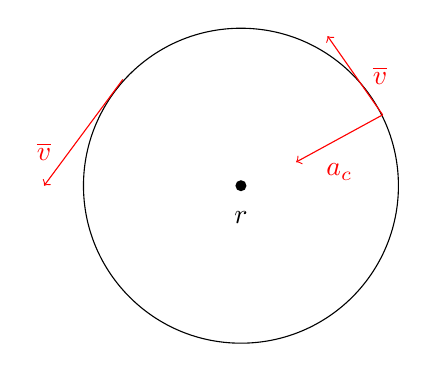
\begin{tikzpicture}
  \fill[black](0,0) circle (2pt) node[below=2mm] {$r$};
  \draw[fill=none](0,0) circle (2.0);
  \draw[red, ->](-1.5,1.35) -- (-2.5,0) node[above=2mm] {$\overline{v}$};
  \draw[red, ->](1.8,0.9) -- (1.1,1.9) node[midway, right=1mm] {$\overline{v}$};
  \draw[red, ->](1.8,0.9) -- (0.7,0.3) node[midway, below=2mm] {$a_c$};
\end{tikzpicture}
\end{figure}

We can define a few variables that relate to this motion. First out is $T$, the \emph{period} in seconds it takes the object to travel along the entire circumference once. Second is the \emph{frequency} $f$, which measures how many times it travels around the circle per second. The two are then inverses, so that $f = 1/T$ and $T = 1/f$.\\
The SI unit for frequency is Hertz; the dimension is then $\text{dim Hertz} = \displaystyle \frac{1}{[T]}$, and $\SI{1}{Hertz} = \SI{1}{s^{-1}}$.

We can consider how fast it moves in a different way, in measuring velocity in \emph{radians per second}, instead of meters per second (or other units of ``regular'' velocity). We call this \emph{angular velocity}, symbol $\omega$. Since there are $2\pi$ radians in a circumference, this implies that

\begin{equation}
\omega = \frac{2 \pi}{T}
\end{equation}

As for the speed $v$ (not the velocity $\vec{v}$ just yet), we can write

\begin{equation}
v = \frac{2 \pi r}{T} = \omega r
\end{equation}


\subsection{Centripetal acceleration}

Note that as the object moves around in a circle, the direction of the velocity vector in constantly changing. This can only happen if there is a nonzero acceleration. This acceleration is called the \emph{centripetal acceleration}, often denoted by $\vec{a_c}$. This acceleration vector always points towards the center of the motion. Because the velocity vector is always tangent to the circle at any given point, the acceleration vector is always perpendicular to the velocity, assuming a constant \emph{speed} around the circle. 

The magnitude of the centripetal acceleration can be stated as

\begin{equation}
|a_c| = \frac{v^2}{r} = \omega^2 r
\end{equation}

\subsubsection{Proportionality of $r$}
Be careful when it comes to the proportionality of $r$. If $T$ is held constant, $v$ is a function of $r$, being equal to

\begin{equation}
v = \frac{2 \pi r}{T}
\end{equation}

and so increasing $r$ will also increase $v$, and thus in the end increase $a_c$:

\begin{equation}
|a_c| = \frac{v^2}{r} = \frac{4 \pi^2 r^2}{r T^2} = \frac{4 \pi^2 r}{T^2}
\end{equation}

Here, it's obvious that increasing $r$ will increase $a_c$, assuming $T$ is held constant. This should come as no surprise, as we are increasing our speed $v$ by moving a longer distance in the same amount of time.

However, let's not fool ourselves into believing that $a_c \propto r$ is always a correct view! Let's now look at the case where we hold the velocity constant (thus changing T) while changing the radius. To get a nice look of how this works, we use the simple equation

\begin{equation}
|a_c| = \frac{v^2}{r}
\end{equation}

Here, holding $v$ constant, it's clear that the centripetal acceleration goes \emph{down} as we increase the radius of the circle we travel in.


\subsection{Planetary orbits}

Let's now have a quick look at the orbits of planets. We will look at them much closer in a few weeks, but until then, let's assume (incorrectly) that orbits are circular. (In reality, they are slightly elliptical.)\\
First out, we have a lecture question:

``The radius of Earth's orbit is $150 \times 10^6$ km. Assuming that the orbit is circular, what is the centripetal acceleration of the Earth?''

They want the answer in $\text{km/yr}^2$, so we shouldn't have to do any ugly conversions.\\
Let's see. The period is one year, by definition (not exactly 365.00 days, but that's another story).

Because $\omega = \frac{2\pi}{T}$ and $T = 1$ year, we find $\omega^2 = 4\pi^2$ radians per year, and $\omega^2 r = (4 \pi^2)(\num{150e6}) = \SI{5.92e9}{km/yr^2}$.

Just to make sure, let's also calculate it using $v^2/r$.

$v$ is found by dividing the circumference of the orbit by the time (1 year), which in then equal in value (but obviously not units) to just the circumference. We then square that, and divide by the radius again; a bit redundant to divide out the radius, but let's go with it for simplicity:

\begin{equation}
v = \frac{2 \pi r}{T} = \frac{2 \pi r}{1 \text{ year}}
\end{equation}

\begin{equation}
a_c = \frac{v^2}{r} = \frac{4 \pi^2 r^2}{r} = 4 \pi^2 r = \SI{5.92e9}{km/yr^2}
\end{equation}

Unsurprisingly, we get the same answer. Still, we have now double-checked, and have also gained a bit of practice doing in two different ways.

Now, let's have a look at the orbits of various planets -- their mean distance to the sun (mean, since the orbits are not truly circular) and periods, and let's compare the centripetal acceleration of various planets. What we find can be seen on this plot below:

\begin{figure}[H]
  \centering
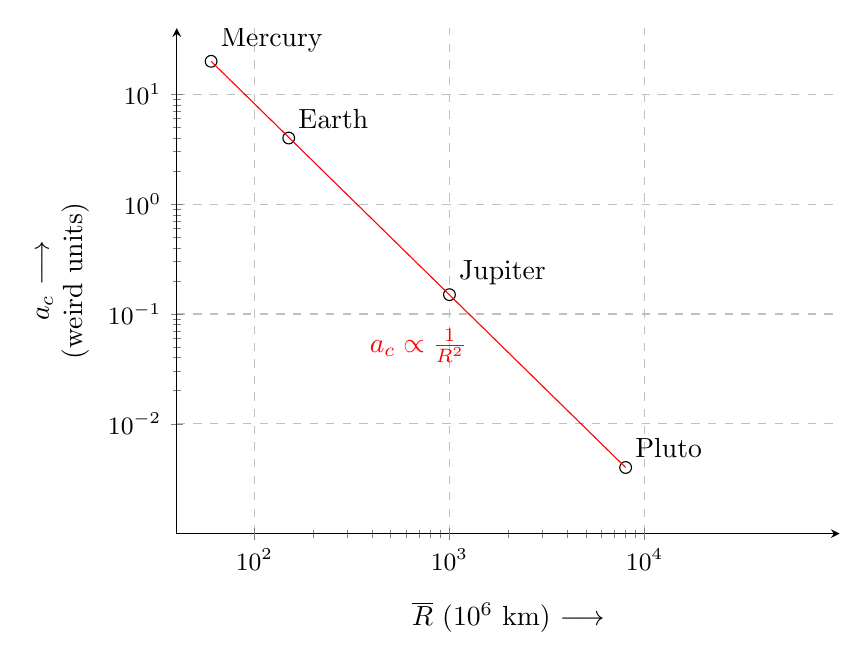
\begin{tikzpicture}
  % Logarithmic plot settings
  \begin{loglogaxis}[
      width=10cm,
      height=8cm,
      xlabel={$\overline{R}$ ($10^6$ km) $\longrightarrow$},
      ylabel style={align=center},
      ylabel={$a_c$ $\longrightarrow$\\(weird units)},
      xmin=4e1, xmax=1e5,
      ymin=1e-3, ymax=4e1,
      xtick={1e2, 1e3, 1e4},
      ytick={1e-2, 1e-1, 1e0, 1e1},
      axis x line=bottom,
      axis y line=left,
      extra x ticks={1e2, 1e3, 1e4},
      extra x tick labels={\phantom{}, \phantom{}, \phantom{}},
      tick label style={font=\small},
      grid=major,
      grid style={dashed, gray!50}
  ]

  % Red line representing ac ∝ 1/R^2
  \addplot[red, thick, domain=1e2:1e4] {1/x^2};

  % Points for planets
  \node[circle, draw=black, fill=white, inner sep=1.5pt] at (axis cs:6e1,2e1) {};
  \node[above right] at (axis cs:6e1,2e1) {Mercury};

  \node[circle, draw=black, fill=white, inner sep=1.5pt] at (axis cs:15e1,4e0) {};
  \node[above right] at (axis cs:15e1,4e0) {Earth};

  \node[circle, draw=black, fill=white, inner sep=1.5pt] at (axis cs:1e3,15e-2) {};
  \node[above right] at (axis cs:1e3,15e-2) {Jupiter};

  \node[circle, draw=black, fill=white, inner sep=1.5pt] at (axis cs:8e3,4e-3) {};
  \node[above right] at (axis cs:8e3,4e-3) {Pluto};

  % Annotation for the red line
  \draw[red] (axis cs:6e1,2e1) -- (axis cs:8e3,4e-3) node[midway, below=7mm] {$a_c \propto \frac{1}{R^2}$};

  \end{loglogaxis}
\end{tikzpicture}
\end{figure}


(It's a bit fun to note that Pluto was still considered a planet when the lecture was recorded! Little has changed in classical mechanics since then, but that one thing certainly has.)

Here, we see the centripetal acceleration on the vertical axis, and the mean distance to the sun on the horizontal. It's clear that the $1/R^2$ fit is rather brilliant! The closer a planet is to the sun, the stronger the centripetal acceleration is, and it falls off following the inverse square law.


\subsection{Centrifuges and more on centripetal acceleration}

Let's now look at the rotation of a glass tube, with a marble inside. The glass tube starts out horizontal, with the marble inside it (see the first picture below):

\begin{figure}[H]
  \centering
\begin{subfigure}[b]{0.4\textwidth}
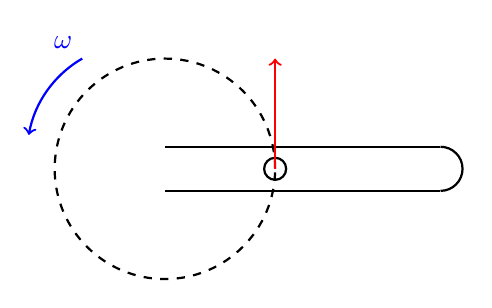
\begin{tikzpicture}[scale=0.7]
  % Draw the dashed circular path
  \draw[dashed, thick] (0,0) circle [radius=2cm];

  \pgfmathsetmacro{\x}{0}
  \pgfmathsetmacro{\r}{0.4}
  \pgfmathsetmacro{\l}{5}

  \draw[thick] (\x,\r) -- (\x+\l,\r);
  \draw[thick] (\x+\l,\r) arc[start angle=90, end angle=-90, radius=\r cm];
  \draw[thick] (\x,-\r) -- (\x+\l,-\r);

  % Draw the small circle at the end of the bar
  \draw[thick] (2,0) circle [radius=0.2cm];

  % Radial arrow (vertical)
  \draw[->, thick, red] (2,0) -- (2,2);

  % Angular velocity arrow
  \draw[->, thick, blue] (-1.5,2) arc[start angle=120, end angle=170, radius=2cm];
  \node[above left, blue] at (-1.5,2) {$\mathbf{\omega}$};

\end{tikzpicture}
\
\end{subfigure}
\begin{subfigure}[b]{0.4\textwidth}
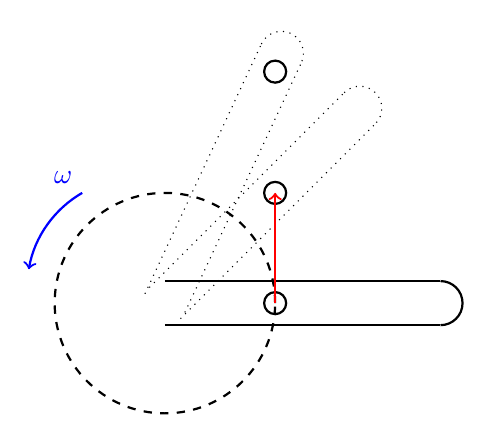
\begin{tikzpicture}[scale=0.7]
  % Draw the dashed circular path
  \draw[dashed, thick] (0,0) circle [radius=2cm];

  \pgfmathsetmacro{\x}{0}
  \pgfmathsetmacro{\r}{0.4}
  \pgfmathsetmacro{\l}{5}

  \draw[thick] (\x,\r) -- (\x+\l,\r);
  \draw[thick] (\x+\l,\r) arc[start angle=90, end angle=-90, radius=\r cm];
  \draw[thick] (\x,-\r) -- (\x+\l,-\r);

  \begin{scope}[rotate around={45:(0,0)}]
  \draw[dotted] (\x,\r) -- (\x+\l,\r);
  \draw[dotted] (\x+\l,\r) arc[start angle=90, end angle=-90, radius=\r cm];
  \draw[dotted] (\x,-\r) -- (\x+\l,-\r);
  \end{scope}

  \begin{scope}[rotate around={65:(0,0)}]
  \draw[dotted] (\x,\r) -- (\x+\l,\r);
  \draw[dotted] (\x+\l,\r) arc[start angle=90, end angle=-90, radius=\r cm];
  \draw[dotted] (\x,-\r) -- (\x+\l,-\r);
  \end{scope}

  % Draw the small circle at the end of the bar
  \draw[thick] (2,0) circle [radius=0.2cm];
  \draw[thick] (2,2) circle [radius=0.2cm];
  \draw[thick] (2,4.2) circle [radius=0.2cm];

  % Radial arrow (vertical)
  \draw[->, thick, red] (2,0) -- (2,2);

  % Angular velocity arrow
  \draw[->, thick, blue] (-1.5,2) arc[start angle=120, end angle=170, radius=2cm];
  \node[above left, blue] at (-1.5,2) {$\mathbf{\omega}$};

\end{tikzpicture}
\end{subfigure}
\end{figure}

Because the glass and the marble are both very smooth, the glass can neither push nor pull on the marble, and so cannot provide any centripetal acceleration. What happens? Well, the glass tube will still rotate, of course -- we assume it's powered by a motor of some kind. The marble, on the other hand, will continue on moving according to its still unchanged velocity vector.

A moment later in time (second picture above), the tube has rotated such that the marble's velocity will take it towards the end of the tube, where we know from experience it will also stay, as long as the tube rotates quickly enough.

\subsection{Artificial gravity through centripetal acceleration}

Let's now look at ``perceived gravity'', or artificial gravity.

\begin{figure}[H]
  \centering
\begin{subfigure}[b]{0.4\textwidth}
  \centering
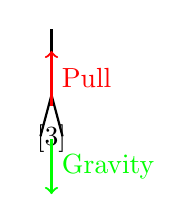
\begin{tikzpicture}[scale=0.7]

  \node at (0, 0) {\Strichmaxerl[3]};
  \draw[thick] (-0.2,0.05) -- (0,0.8);
  \draw[thick] (0.2,0.05) -- (0,0.8);
  \draw[thick] (0,0.8) -- (0,2);
  \draw[thick, red, ->] (0,0.6) -- (0,1.6) node[midway, right] {Pull};
  \draw[thick, green, ->] (0,0) -- (0,-1) node[midway, right] {Gravity};

\end{tikzpicture}
\end{subfigure}
\
\begin{subfigure}[b]{0.4\textwidth}
  \centering
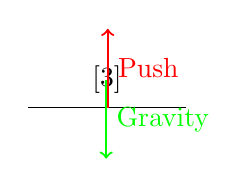
\begin{tikzpicture}[scale=1]

  \node at (0, 0) {\Strichmaxerl[3]};
  \draw (-1,-0.35) -- (1,-0.35);
  \draw[thick, red, ->] (0.01,-0.35) -- (0.01,0.65) node[midway, right] {Push};
  \draw[thick, green, ->] (-0.01,0) -- (-0.01,-1) node[midway, right] {Gravity};

\end{tikzpicture}
\end{subfigure}
\end{figure}
As the illustration shows, we will always experience gravity opposite to any pull or push. The same is true if we somehow hang on to a rope and spin around -- or ride a merry-go-round or something to that effect. We will have a centripetal force inwards, and feel a ``pull'' inwards, but perceive gravity in exactly the opposite direction, as if we were drawn outwards.

Let us now consider a large, circular space station, which experiences almost no gravity (as it is in orbit, essentially in perpetual free fall). It is a big ``wheel'', with a radius of 100 m. We want the centripetal acceleration to be about \SI{10}{m/s^2} for a person standing on the outer wall. How fast should it rotate (what should be the period)?

\begin{figure}[H]
  \centering
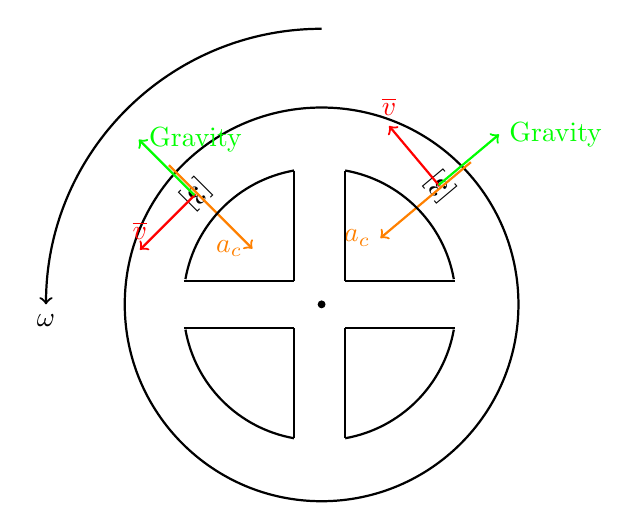
\begin{tikzpicture}[scale=1]

  \draw[thick] (2,0) circle [radius=25mm];
  \fill (2,0) circle [radius=0.5mm];

  \pgfmathsetmacro{\rotate}{130}
  \begin{scope}[xshift=35mm, yshift=15mm]
  \begin{scope}[rotate=\rotate]
    \node at (0, 0) {\rotatebox{\rotate}{\Strichmaxerl[3]}};
    \draw[thick, orange, ->] (-0.02,-0.5) -- (-0.02,1) node[left] {$a_c$};
    \draw[thick, red, ->] (0,0) -- (1,0) node[above] {$\overline{v}$};
    \draw[thick, green, ->] (0.02,0) -- (0.02,-1) node[right] {Gravity};
  \end{scope}
  \end{scope}

  \pgfmathsetmacro{\rotate}{-135}
  \begin{scope}[xshift=4mm, yshift=14mm]
  \begin{scope}[rotate=\rotate]
    \node at (0, 0) {\rotatebox{\rotate}{\Strichmaxerl[3]}};
    \draw[thick, orange, ->] (-0.02,-0.5) -- (-0.02,1) node[left] {$a_c$};
    \draw[thick, red, ->] (0,0) -- (1,0) node[above] {$\overline{v}$};
    \draw[thick, green, ->] (0.02,0) -- (0.02,-1) node[right] {Gravity};
  \end{scope}
  \end{scope}

  \draw[thick, ->] (2,3.5) arc[start angle=90, end angle=180, radius=35mm] node[below] {$\omega$};

  \draw[thick] (1.65,1.7) arc[start angle=100, end angle=170, radius=17mm];
  \draw[thick] (2.30,1.7) arc[start angle=80, end angle=10, radius=17mm];
  \draw[thick] (2.30,-1.7) arc[start angle=-80, end angle=-10, radius=17mm];
  \draw[thick] (1.65,-1.7) arc[start angle=-100, end angle=-170, radius=17mm];

  \draw[thick] (1.65,-1.7) -- (1.65, -0.3);
  \draw[thick] (1.65,1.7) -- (1.65, 0.3);
  \draw[thick] (2.30,1.7) -- (2.30, 0.3);
  \draw[thick] (2.30,-1.7) -- (2.30, -0.3);

  \draw[thick] (0.25,0.3) -- (1.65,0.3);
  \draw[thick] (0.25,-0.3) -- (1.65,-0.3);
  \draw[thick] (2.30,-0.3) -- (3.70,-0.3);
  \draw[thick] (2.30,0.3) -- (3.70,0.3);

\end{tikzpicture}
\end{figure}

We can use $\omega^2 r$ here; it should equal \SI{10}{m/s^2}, so we find

\begin{align}
(\omega^2)(\SI{100}{m}) &= \SI{10}{m/s^2}\\
\omega^2 &= \frac{\SI{10}{m/s^2}}{\SI{100}{m}}\\
\omega^2 &= \SI{0.1}{rad^2/s^2}\\
\omega &= \sqrt{0.1} \text{ rad/s}
\end{align}

And, because $\omega = \frac{2 \pi}{T}$:

\begin{align}
\frac{2 \pi}{T} &= \sqrt{0.1}\\
T &= \frac{2 \pi}{\sqrt{0.1}} \approx \SI{20}{s}
\end{align}

So if we rotated the space station with a period of about/just over 20 seconds, we would perceive it as if we had Earth's gravity.

The gravitational acceleration is zero at the center, but it grows as you come closer to the outer edge. If you were to ``jump'' down the shaft, you would end up crashing into the outer wall at a velocity great enough that you may well be killed!


\section{Lecture 6: Newton's first, second, and third laws}

In this lecture, we will introduce the concept of \emph{force}, an extremely important quantity in physics. Last lecture used forces, but referred to them as ``pushes'' or ``pulls''. We will now start using the correct terminology.

\subsection{Newton's first law}

Newton's first law essentially dates back to Galileo Galilei, in his ``law of inertia''.\\
Newton wrote it as

\begin{quote}
Every body perseveres in its state of rest, or uniform motion in a right line, unless it is compelled to change that state by forces impressed upon it.
\end{quote}

This means that if we perceive ourselves to be at rest unless we experience an unbalanced force such as an acceleration
of a car we are in. We do experience forces we stand still: the gravitational force and the normal force. However,
those cancel each other out.

Newton's first law, however, is not valid in all reference frames. It is only valid in inertial references frames, the definition of which is a reference frame where the motion of a particle not under any forces moves in a straight line at constant speed. In particular, this is not true in a reference frame which is being accelerated in any way.

So the question is: can we find an inertial reference frame? Is the lecture hall an inertial reference frame, for example?\\
In can't be. The Earth spins, causing a centripetal acceleration. That's an acceleration, so the answer is already no. There are many additional reasons, though: the Earth moves around the Sun, again causing centripetal acceleration. The Sun moves around the galaxy's center, the galaxy itself has an orbit, and so on.

The Earth has, as mentioned, a centripetal acceleration. We can estimate it by calculating $\omega^2 R_{earth}$, which turns out to be about \SI{0.034}{m/s^2}, which is of course much, much lower than the acceleration due to gravity. If the Earth spun much, much faster, the centripetal acceleration might start to cancel out gravity noticeably, however.

Let's then calculate the centripetal acceleration due to the orbit around the Sun. The radius of the orbit is about $\SI{150e9}{m}$, and the period is of course one year.

\begin{align}
\omega &= \frac{2 \pi}{T} = \frac{2 \pi}{365 \cdot 24 \cdot 60 \cdot 60} = \SI{1.992e-7}{rad/s}\\
a_c = \omega^2 r &= (\SI{1.992e-7}{rad/s})^2 \times \SI{150e9}{m} = \SI{5.95e-3}{m/s^2}
\end{align}

Because the centripetal accelerations calculated above are so tiny, we can consider the Earth as being very close to an inertial reference frame.

A mathematical statement of Newton's first law might be

\begin{equation}
\sum \vec{F} = 0 \Rightarrow \frac{d\vec{v}}{dt} = 0 \text{ (Newton's first law)} \label{eq:newton1}
\end{equation}

\subsection{Newton's second law}

Say we have a spring (though the law isn't specific to springs), in the absence of gravity. We extend the spring, and attach a mass $m_1$ at the end of the spring.

\begin{figure}[H]
     \centering
\begin{tikzpicture}
     % Draw a spring
     \draw[decorate, decoration={aspect=0.5, segment length=5mm, amplitude=3.5mm, coil}] 
         (0,0) -- (5,0);
     \fill[black] (5,0) circle (3mm) node[above right = 3mm and 2mm] {$m_1$};
     \draw[thick] (0,-1) -- (0,1);
     \draw[thick, red, -{Stealth[scale=1.5]}] (5,0) -- (3,0) node[midway, above = 4mm] {pull};
     \draw[dotted] (2.4, -1) -- (2.4, 1);
 \end{tikzpicture}
\end{figure}

Immediately after we let go of the mass, so that the spring's ``pull'' contracts the spring and pulls the mass with it, we measure the acceleration of the mass to be $a_1$.\\
We then replace the mass with another mass $m_2$, and measure the acceleration, in the same manner, to be $a_2$.

We will then find that $m_1 a_1 = m_2 a_2$. The product $m a$ is the \emph{force} (which we have called a ``push'' or a ``pull'' until now) exerted upon the mass by the spring. The spring's force is independent on the mass, but the acceleration caused on the mass is not; the acceleration is inversely proportional to the mass.

In equation form, Newton's second law -- one of the most important equations in physics -- reads

\begin{equation}
\vec{F} = m \vec{a} \text{ (Newton's second law)} \label{eq:newton2}
\end{equation}

As shown above, force is a vector. The direction of the acceleration caused by a force is always in the same direction as the force.

The SI unit for force is the newton, in honor of Newton himself, of course. Because the product $m a$ is in units of $\displaystyle \text{kg} \cdot \frac{\text{m}}{\text{s}^2}$, 1 newton equals 1 $\displaystyle \text{kg} \cdot \frac{\text{m}}{\text{s}^2}$.

Just as with the first law, we cannot truly prove Newton's second law. Like the first, it is only valid in inertial reference frames, and we cannot provide such a reference frame to conduct our experiments in.

Note that no statement is made regarding speed or velocity, only acceleration. The law holds equally well at 0 m/s, 5 m/s and 5000 m/s. However, once speeds start becoming noteworthy in relation to the speed of light, Newtonian mechanics becomes more and more inaccurate, and we instead need to use Einstein's relativity for accurate results. 

\subsection{Newton's third law}

Let's now have a look at the gravitational force. Using the second law, we see that the force is equal to $m \vec{g}$. Double the mass, double the force, etc.\\
We assume that the lecture hall is an inertial reference frame. Consider an object that is at rest (relative to the lecture hall). We know from the above that there must be a gravitational force on the object, pulling it downwards. However, it is at rest, so there is no acceleration (in our reference frame). Therefore, the net force on it \emph{must} be zero. This is only possible, of course, if there is an equal and opposite force -- or sums of forces that adds up to exactly cancel the gravitational force out.

The above is the result of the third law, which can be stated as

\begin{quote}
If one object exerts a force on another, the other exerts the same force in the opposite direction on the one.
\end{quote}

In other words, if gravity pulls you down into your chair with a force of, say, 700 N, then the chair exerts a force of 700 N back on you. It can be stated more simply as $\text{action} = -\text{reaction}$.\\
We can therefore also write the law as

\begin{equation}
\vec{F_{12}} = -\vec{F_{21}} \text{ (Newton's third law)} \label{eq:newton3}
\end{equation}

where $\vec{F_{ab}}$ means the force exerted \emph{by} object a \emph{on} object b. Note that some physics textbook authors use the reverse notation, which can get confusing.

Unlike the first and second laws, the third laws always holds, including in accelerated reference frames.


\subsection{Examples of Newton's laws in use}

Let's look at a few examples of Newton's law in practice.

\begin{figure}[H]
     \centering
\begin{tikzpicture}

     \draw[thick] (0,0) rectangle (1,1) node[midway] {$1$} node[midway, above=9mm] {$m_1=5$};
     \draw[thick] (1,-0.5) rectangle (3,1.5) node[midway] {$2$} node[midway, above=10mm] {$m_2=15$};

     \draw[thick, red, -{Stealth[scale=1.5]}] (-2,0.5) -- (0,0.5) node[above left=4mm] {$\overline{F}=20$};
 \end{tikzpicture}
\end{figure}



There's a force of 20 newtons towards the right, as shown. Because the total mass is 20 kg, and the force is 20 newton, there will be an acceleration of $\SI{1}{m/s^2}$ via $\displaystyle \vec{a} = \frac{\vec{F}}{m}$ -- Newton's second law. If not else, we know from intuition and daily life that both objects will move towards the right together, with the same acceleration (and thus velocity, since they started together), once they start moving.

The entirety of the force is on object 1. Since they move together, there must be a force between object 1 and object 2 ($\vec{F_{12}}$), towards the right, or object two could not accelerate.

Since we know that the force on object 1 from the left is 20 N, and we also know that $m_1 = \SI{5}{kg}$ and $a_1 = \SI{1}{m/s^2}$ to the right, we can use Newton's second law to find the net force on object 1 to be 5 N towards the right, despite the force on it from the left being 20 N.

How come? Well, the answer lies in object 2. We know that $m_2 = \SI{15}{kg}$ and $a_2 = \SI{1}{m/s^2}$, so the net force on object 2 \emph{must} be 15 N towards the right. The \emph{only} force on object 2 is $\vec{F_{12}}$, so that too must be 15 N towards the right.

What about object 1? Well, Because of $\vec{F_{12}}$ being 15 N to the right, there must be a force $\vec{F_{21}}$ of 15 N towards the left, back on object 1, which ``cancels out'' most of the 20 N, and leaves object 1 with a net 5 N force to the right. In math form:

\begin{equation}
\vec{F_1} = \vec{F} + \vec{F_{21}} = +20\hat{x} + (-15\hat{x}) = +5 \hat{x}
\end{equation}

... defining the increasing direction of $x$ being towards the right.

Now, what about the sum of forces on object 2? Don't we have 15 N towards the right from object 1, and 15 N towards the left back to object 1, for a net zero force? No! The fact that $a \neq 0$ is enough to prove that this cannot be the case.

It's important to note and understand that the two forces $\vec{F_{12}}$ and $\vec{F_{21}}$ act on different bodies. They don't cancel each other out on an individual object. $\vec{F_{21}}$ is a force that object 2 exerts on object 1 -- that fact does \emph{not} in any way negate the force exerted by 1 on 2! If that were the case, object 2 could not accelerate, since its net force would be zero.


\subsection{Tension and another example of Newton's laws in use}

Say we hang a mass $m$ from two strings, suspended at different heights. The leftmost string makes an angle of 45 degrees with the roof above, while the rightmost string makes an angle of 60 degrees. We call the tension in the rightmost string $T_1$, and in the leftmost $T_2$. We consider increasing $x$ to be towards the right, and increasing $y$ to be upwards.

\begin{figure}[H]
     \centering
\begin{tikzpicture}
     \draw (0,2) -- (2,0);
     \draw (2,0) -- (3,2);
     \draw[thick] (-1,2) -- (4,2);
     \draw[thick, red, -{Stealth[scale=1.5]}] (2,0) -- (1.5,0.5) node[below = 4mm] {$T_2$};
     \draw[thick, red, -{Stealth[scale=1.5]}] (2,0) -- (2.5,1) node[below = 4mm] {$T_1$};
     \draw[thick, red, -{Stealth[scale=1.5]}] (2,0) -- (2,-1.5) node[below = 2mm] {$mg$};
     \draw[dotted, -{Stealth[scale=1.5]}] (-1,0) -- (-1,1) node[midway, right = 2mm] {$+y$};
     \draw[-{Stealth[scale=1.5]}] (3,-0.5) -- (4,-0.5) node[below = 2mm] {$+x$};
     \draw[dotted] (0,0) -- (4,0);
 \end{tikzpicture}
\end{figure}


There will be a gravitational force of magnitude $m g$ downwards. Because the object is in equilibrium, sitting still with no acceleration, the \emph{net force} on the object must be zero -- that is clear from Newton's second law.\\
Therefore, we conclude that the two tensions $T_1$ and $T_2$ perfectly balance the gravitational force $m g$, so that the net force on the object is zero.

Force is a vector, so we can decompose this into two one-dimensional problems. We don't need to decompose the gravitational force, of course: it is already only in the $-y$ direction. Let's decompose the tension vectors, though.

Let's start with $T_1$. It makes a 60 degree angle with the horizontal, so by using vector decomposition, we find

\begin{align}
T_{1x} &= T_1 \cos(\ang{60}) = \frac{T_1}{2}\\
T_{1y} &= T_1 \sin(\ang{60}) = \frac{T_1 \sqrt{3}}{2}
\end{align}

As for $T_2$, it makes a 45 degree angle, so the sine and cosine are both one over the square root of two. (It makes sense that the force is equal in both directions, since the angle is exactly in the middle of a 90 degree angle, so to speak.)

\begin{align}
T_{2x} &= T_2 \cos(\ang{45}) = \frac{T_2}{\sqrt{2}}\\
T_{2y} &= T_2 \sin(\ang{45}) = \frac{T_2}{\sqrt{2}}
\end{align}

What then? Well, we know that the net force must be zero, since there is no acceleration. The same can be said for each axis independently, too: $\sum F_x = 0$ and $\sum F_y = 0$. We can set up equations representing this:

\begin{align}
T_{1x} + T_{2x} = 0\\
\frac{T_1}{2} - \frac{T_2}{\sqrt{2}} = 0\\
T_1 = \frac{2 T_2}{\sqrt{2}} = \sqrt{2} \cdot T_2 \label{eq:lec6_t1}
\end{align}

Note that because $T_2$ points towards the negative $x$ direction, the sum of these two forces becomes a subtraction.

As for the $y$ axis:

\begin{align}
T_{1y} + T_{2y} = m g\\
\frac{T_1 \sqrt{3}}{2} + \frac{T_2}{\sqrt{2}} = m g\\
T_2 = \sqrt{2}\left(m g - \frac{T_1 \sqrt{3}}{2}\right)
\end{align}

Alternatively, we could have written $T_{1y} + T_{2y} - m g = 0$ (minus $m g$ since it is in the opposite direction) to show that the sum is zero, rather than saying that they must be equal. This is of course the same thing algebraically.

We now have two equations with two unknowns. Let's substitute the value of $T_1$ into the second equation from \eqref{eq:lec6_t1} and find $T_2$ as a function of only $m$ and constants:

\begin{align}
T_2 = \sqrt{2}\left(m g - \frac{\sqrt{2} T_2 \sqrt{3}}{2}\right)\\
T_2 = \sqrt{2} m g - T_2 \sqrt{3}\\
T_2 + \sqrt{3} T_2 = \sqrt{2} m g\\
T_2 (1 + \sqrt{3}) = \sqrt{2} m g\\
T_2 = \frac{\sqrt{2} m g}{1 + \sqrt{3}}
\end{align}

Since $T_1 = \sqrt{2} T_2$, $T_1$ is simply

\begin{equation}
T_1 = \frac{2 m g}{1 + \sqrt{3}}
\end{equation}

We can finally substitute in some values. The lecture used $m = \SI{4}{kg}$, so let's try that. We find

\begin{align}
T_1 &= \frac{(2)(\SI{4}{kg})(\SI{9.8}{m/s^2})}{1 + \sqrt{3}} \approx \SI{28.7}{N}\\
T_2 &= \frac{T_1}{\sqrt{2}} \approx \SI{20.3}{N}
\end{align}

The professor's answers differ slightly, but match up perfectly if we use $g = \SI{10}{m/s^2}$, so he most likely used that approximation.

As a sanity check, and additional practice, let's just make sure that the forces indeed balance out.

\begin{align}
T_1 \cos(\ang{60}) - T_2 \cos(\ang{45}) &\overset{?}{=} 0\\
14.35 - 14.35 &= 0
\end{align}

... so that indeed works out in the $x$ direction. Let's check $y$:

\begin{align}
T_1 \sin(\ang{60}) + T_2 \sin(\ang{45}) &\overset{?}{=} m g\\
24.85 + 14.35 &= 39.2
\end{align}

It works out perfectly!

%%% Local Variables:
%%% TeX-master: "../../main"
%%% End:
